%%% LaTeX Template: Designer's CV
%%%
%%% Source: http://www.howtotex.com/
%%% Feel free to distribute this template, but please keep the referal to HowToTeX.com.
%%% Date: March 2012


%%%%%%%%%%%%%%%%%%%%%%%%%%%%%%%%%%%%%
% Document properties and packages
%%%%%%%%%%%%%%%%%%%%%%%%%%%%%%%%%%%%%
\documentclass[a4paper,11pt,final]{memoir}

% misc
\renewcommand{\familydefault}{bch}	% font
\pagestyle{empty}					% no pagenumbering
\setlength{\parindent}{0pt}			% no paragraph indentation


% required packages (add your own)
\usepackage{flowfram}										% column layout
\usepackage[top=1cm,left=1cm,right=1cm,bottom=1cm]{geometry}% margins
\usepackage{graphicx}										% figures
\usepackage{url}											% URLs
\usepackage[usenames,dvipsnames]{xcolor}					% color
\usepackage{multicol}										% columns env.
	\setlength{\multicolsep}{0pt}
\usepackage{paralist}										% compact lists
\usepackage{tikz}

\usepackage[czech]{babel}
\usepackage[utf8x]{inputenc}
\usepackage[T1]{fontenc}

\usepackage{hyperref}
\hypersetup{colorlinks=true, urlcolor=blue}

%%%%%%%%%%%%%%%%%%%%%%%%%%%%%%%%%%%%%
% Create column layout
%%%%%%%%%%%%%%%%%%%%%%%%%%%%%%%%%%%%%
% define length commands
\setlength{\vcolumnsep}{\baselineskip}
\setlength{\columnsep}{\vcolumnsep}

% frame setup (flowfram package)
% left frame
\newflowframe{0.24\textwidth}{\textheight}{0pt}{0pt}[left]
	\newlength{\LeftMainSep}
	\setlength{\LeftMainSep}{0.24\textwidth}
	\addtolength{\LeftMainSep}{2\columnsep}
% right frame
\newflowframe{0.7\textwidth}{\textheight}{\LeftMainSep}{0pt}[main01]

% horizontal rule between frames (using TikZ)
\renewcommand{\ffvrule}[3]{%
\hfill
\tikz{%
	\draw[loosely dotted,color=RoyalBlue,line width=1.5pt,yshift=-#1] 
	(0,0) -- (0pt,#3);}%
\hfill\mbox{}}
\insertvrule{flow}{1}{flow}{2}


%%%%%%%%%%%%%%%%%%%%%%%%%%%%%%%%%%%%%
% define macros (for convience)
%%%%%%%%%%%%%%%%%%%%%%%%%%%%%%%%%%%%%
\newcommand{\Sep}{\vspace{1.4em}}
\newcommand{\SmallSep}{\vspace{0.7em}}

\newenvironment{AboutMe}
	{\ignorespaces\textbf{\color{RoyalBlue} About me}}
	{\Sep\ignorespacesafterend}
	
\newcommand{\CVSection}[1]
	{\Large\textbf{#1}\par
	\SmallSep\normalsize\normalfont}

\newcommand{\CVItem}[1]
	{\textbf{\color{RoyalBlue} #1}}


%%%%%%%%%%%%%%%%%%%%%%%%%%%%%%%%%%%%%
% Begin document
%%%%%%%%%%%%%%%%%%%%%%%%%%%%%%%%%%%%%
\begin{document}

% Left frame
%%%%%%%%%%%%%%%%%%%%
\begin{figure}
	\hfill
	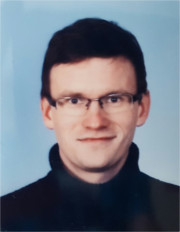
\includegraphics[width=0.7\columnwidth]{photo.jpg}
	\vspace{-7.5cm}
\end{figure}

\begin{flushright}\small
	Dušan Rychnovský \\
	\url{rychnovskyd@gmail.com}  \\
	\url{www.dusanrychnovsky.cz} \\
	(+420) 705 224 922
\end{flushright}\normalsize
\framebreak


% Right frame
%%%%%%%%%%%%%%%%%%%%
\Huge\bfseries {\color{RoyalBlue} Dušan Rychnovský} \\
\Large\bfseries  Software engineer \\

\normalsize\normalfont

% About me
\begin{AboutMe}
I am a software engineer with many years of experience, mostly in Java, distributed computing and C\#/Azure. My biggest strengths are analytical thinking, proficiency with software engineering tools and practices and background in computer science.

\medskip
You can find me at 
\href{http://cz.linkedin.com/pub/du%C5%A1an-rychnovsk%C3%BD/96/a42/a0/}{LinkedIn}.
You might also be interested in my
\href{http://stackoverflow.com/users/1103412/dusan-rychnovsky}{Stack Overflow} and
\href{https://github.com/dusan-rychnovsky}{GitHub} accounts and my
\href{http://blog.dusanrychnovsky.cz}{technical blog}.
\end{AboutMe}

% Experience
\CVSection{Experience}

\CVItem{Microsoft, 2017 - current}\\
Working on Dynamics Marketing, a successful marketing automation platform, which allows to elevate customer experiences and orchestrate personalized journeys across all touchpoints.

I played a major role in implementing the lead scoring and consent management systems, and in maintaining an in-house distributed computing platform, including requirements and technical design, assuring quality, continuous integration and deployment and a 24/7 livesite rotation.

\vspace{0.2em}
\textit{C\#, Azure, Kubernetes, Azure Devops}
\SmallSep

\CVItem{Seznam.cz, 2015 - 2017}\\
Working on Robot, web crawling component of Seznam's fulltext-search engine, which maintains an index of multiple bilion most interesting web pages and images from all over the Internet.

I incorporated neural networks for image-content recognition, speeded
up link-analysis based signals calculation and ported it onto a new
platform, added support for videos to the system for fast crawling
of fresh content (such as news-sites).

\vspace{0.2em}
\textit{Java, Hadoop, Spark, HBase, Euphoria, Akka, GIT, Maven, Linux}
\SmallSep

\CVItem{Casenet, 2014 - 2015}\\
Working on TruCare, an enterprise-level care management system used
by large US health maintenance organizations.

I took part in building a REST API for mobile and other external clients
and in the development of a platform for extending the application with
third-party correspondence systems.

\vspace{0.2em}
\textit{Java, Spring, Hibernate, Jersey, GIT, Maven}
\SmallSep

\CVItem{X-Center, 2011 - 2014}\\
Working on an ECM solution used by many large hospitals, insurance companies, etc. from around the world.

\vspace{0.2em}
\textit{Java, OpenText technologies, SVN, Maven}
\Sep

% Education
\CVSection{Education}
\CVItem{2011 - 2014}\\
M.S in Software Engineering at the Faculty of Mathematics and Physics, Charles University in Prague\\
\SmallSep
Master Thesis: \href{http://www.dusanrychnovsky.cz/files/master-thesis.pdf}{Generating of Synthetic XML Data}
\SmallSep

\CVItem{2008 - 2011}\\
B.S. in Computer Science at the Faculty of Mathematics and Physics, Charles University in Prague
\Sep

% Skills
\CVSection{Skills}

\CVItem{Java}\\
Java, Spring, Hibernate, Akka,
\SmallSep

\CVItem{Distributed Computing}\\
HDFS, Hadoop Map-Reduce, HBase, Apache Spark, Euphoria
\SmallSep

\CVItem{Azure}\\
C\#, Kubernetes, Blob Storage, Cosmos DB, Azure Devops
\SmallSep

\CVItem{Build Tools \& Versioning Systems}\\
Maven, Git,
\SmallSep 

\CVItem{Languages}\\
Czech (native speaker), English (fluent), German (basic).
\Sep 

%%%%%%%%%%%%%%%%%%%%%%%%%%%%%%%%%%%%%
% End document
%%%%%%%%%%%%%%%%%%%%%%%%%%%%%%%%%%%%%
\end{document}
